\documentclass[14pt, openany, titlepage]{report} % Explicitly use openany and titlepage
\usepackage[utf8]{inputenc}
\usepackage[italian,english]{babel}
\usepackage{graphicx}
\usepackage{cite}
\usepackage{amsmath}
\usepackage[table,xcdraw]{xcolor}
\usepackage[italian]{minitoc}
\usepackage{fancybox}
\usepackage{fancyhdr}
\usepackage{verbatim}
\usepackage{url}
\usepackage{color}
\usepackage{listings}
\usepackage{makeidx}
\usepackage{comment}
\usepackage{hyperref}
\usepackage{bm}
\usepackage{longtable}
\usepackage{tabularx}
\usepackage{placeins}
\usepackage{caption}
\usepackage{float}
\usepackage{xcolor}
\usepackage{soul}
\usepackage{array}
\usepackage{multirow}
\usepackage{adjustbox} % Pacchetto per ridimensionare automaticamente
\usepackage{graphicx} % Per il ridimensionamento
\usepackage{lscape}
\usepackage{mathtools}
\usepackage{amsmath}
\usepackage{amssymb}
\usepackage{listings}
\usepackage[svgnames]{xcolor}
\usepackage{booktabs}

% Set link colors without borders
\hypersetup{
    colorlinks=true,
    linkcolor=black,
    filecolor=magenta,      
    urlcolor=cyan,
}

\lstset{frame=tb,
    language=Java,
    numbers=left,
    keywordstyle=\color{blue},
    alsoletter={.}
}

\lstset{language=R,
    basicstyle=\small\ttfamily,
    stringstyle=\color{DarkGreen},
    otherkeywords={0,1,2,3,4,5,6,7,8,9},
    morekeywords={TRUE,FALSE},
    deletekeywords={data,frame,length,as,character},
    keywordstyle=\color{blue},
    commentstyle=\color{DarkGreen},
}

\graphicspath{ {./Figure/} }


% Minimize additional blank pages
\let\cleardoublepage\clearpage % Suppresses new page on odd side
\flushbottom % Avoid vertical blank space between paragraphs

% Title Page
\begin{document}
\selectlanguage{italian}

\begin{titlepage}
\begin{center}
    \begin{figure}
        
\includegraphics[width=3.5cm, height=3.5cm]{unisa.png}
        \centering
    \end{figure}
    {\Large Università degli Studi di Salerno}\\[0.2truecm]
    {\large Dipartimento di Informatica\\Corso di Laurea Triennale in Informatica}\\
    \hrulefill
    \vfill
    {\large Progetto Calcolo Probabilità Statistica Matematica\\(CPSM)}\\[0.1truecm]
    \vfill\vfill
    {\LARGE {\bf Indagine Statistica sulle\\[0.1truecm]Morti in incidenti stradali}}
    \vfill\vfill
    
    \hfill  \textbf{Tozza Gennaro Carmine}
    \centerline{\hfill Matricola: 0512120382}
    
    \vfill
    \hrulefill 
    \begin{center} Anno Accademico 2024-2025 \end{center}
\end{center}
\end{titlepage}

% Suppress page break after table of contents
\tableofcontents

\chapter{Introduzione}
\section{Problematica}
Gli \textbf{incidenti stradali} costituiscono una delle principali emergenze 
di sanità pubblica, in quanto responsabili ogni anno di un elevato 
numero di decessi, in particolare tra i giovani, e di gravi conseguenze
 in termini di disabilità temporanee e permanenti, oltre al drammatico impatto umano e psicologico sulle vittime e 
 sulle loro famiglie. 
\noindent

\section{Scopo del progetto}
Il progetto consiste nel realizzare un’indagine statistica \footnote{\url{https://siqual.istat.it/SIQual/visualizza.do?id=7777778&refresh=true&language=IT}}sugli incidenti stradali verificatisi sulla rete stradale del territorio nazionale, tra il 2010 e il 2023 verbalizzati da un'autorità di Polizia o dai Carabinieri, 
avvenuti su una strada aperta alla circolazione pubblica e che hanno causato morti (entro il 30° giorno) con il coinvolgimento 
di almeno un veicolo. \\\\
\noindent
La rilevazione è condotta correntemente dall’Istat, con la compartecipazione dell'ACI e di numerosi Enti pubblici istituzionali, 
è a carattere totale e a cadenza mensile (inserita tra le rilevazioni di interesse pubblico nel Programma Statistico Nazionale - PSN - IST00142). \\\\
\noindent
Per l'analisi dei dati è stato scelto l'ambiente di calcolo statistico \textbf{R}. \\
R fornisce un'ampia varietà di tecniche statistiche (modellazione lineare e non lineare, test statistici classici, analisi delle serie temporali, classificazione, \dots)
e grafiche ed è altamente estensibile.\\\\
\noindent
Uno dei punti di forza di R è la facilità con cui possono essere prodotti grafici ben progettati e di qualità per la pubblicazione, 
compresi simboli matematici e formule se necessario.\\\\
\noindent
Per semplificare l'analisi, si è scelto di lavorare non sull'intero dataset, 
ma su un sottoinsieme filtrato di dati, relativo alle morti per incidenti stradali che riguardano solo i conducenti di età compresa tra i 21 e i 24 anni.\\\\
\noindent
Per approfondire l'analisi con dati dettagliati e specifici, è possibile consultare il dataset direttamente sul sito dell'ISTAT al seguente link:
\url{https://esploradati.istat.it/databrowser/#/it/dw/categories/IT1,Z0810HEA,1.0/HEA_ROAD/IT1,41_270_DF_DCIS_MORTIFERITISTR1_1,1.0}\\\\
\noindent
Il dataset in formato CSV(Comma-Separated Values) è stato ottenuto dalla fonte ISTAT tramite il link indicato, assicurando così l'affidabilità dei dati.\\\\
Il formato scelto (CSV) permette un'agevole manipolazione dei dati, essendo compatibile con la maggior parte dei software statistici e
dei fogli di calcolo, ottimizzando l'analisi e la visualizzazione delle informazioni.\\

\begin{table}[!ht]
\centering
\footnotesize
\begin{tabularx}{\textwidth}{|l|*{14}{>{\centering\arraybackslash}X|}}
\hline
\textbf{Intersezione} & \textbf{'10} & \textbf{'11} & \textbf{'12} & \textbf{'13} & \textbf{'14} & \textbf{'15} & \textbf{'16} & \textbf{'17} & \textbf{'18} & \textbf{'19} & \textbf{'20} & \textbf{'21} & \textbf{'22} & \textbf{'23} \\ 
\hline
Incrocio & 55 & 45 & 42 & 23 & 34 & 24 & 28 & 25 & 23 & 13 & 15 & 16 & 21 & 10 \\ \hline
Rotatoria & 7 & 4 & 2 & 5 & 5 & 1 & 5 & 3 & 1 & 2 & 1 & 2 & -- & 3 \\ \hline
Rettilineo & 92 & 102 & 89 & 82 & 96 & 95 & 66 & 70 & 60 & 72 & 66 & 69 & 69 & 74 \\ \hline
Curva & 58 & 51 & 48 & 46 & 45 & 44 & 41 & 36 & 38 & 42 & 23 & 40 & 27 & 38 \\ \hline
Dosso/Pend. & 2 & 7 & 2 & 4 & 2 & 3 & 5 & 1 & 2 & 3 & 2 & 4 & 3 & 1 \\ \hline
Galleria & 1 & 1 & 1 & 1 & -- & 1 & 1 & 1 & -- & -- & 3 & 1 & -- & -- \\ \hline
\hline
\textbf{Totale} & 215 & 210 & 184 & 161 & 182 & 168 & 146 & 136 & 124 & 132 & 110 & 132 & 120 & 126 \\ \hline
\end{tabularx}
\end{table}

\normalsize


\chapter{Tabelle delle frequenze}

\begin{center}
\begin{lstlisting}[breaklines=true]
# inclusione librerie
library("tidyverse")
require("tidyverse")
library("dplyr")

# viene caricato il dataset
dati <- read.csv("dati_istat.csv")

# filtraggio dati
dati <- dati %>% select(Intersezione, TIME_PERIOD, Osservazione) 
dati <- dati %>% 
  filter(Intersezione != "Totale") 

# 1. Frequenze assolute per intersezione dell'incidente
freq_assolute <- aggregate(Osservazione ~ Intersezione, data=dati, sum)
colnames(freq_assolute) <- c("Intersezione", "Frequenza_Assoluta")
print(freq_assolute)

# 2. Frequenze relative per intersezione dell'incidente
totale <- sum(freq_assolute$Frequenza_Assoluta)
freq_assolute$Frequenza_Relativa <- freq_assolute$Frequenza_Assoluta / totale
print(freq_assolute)

# 3. Frequenze cumulate assolute
freq_assolute <- freq_assolute[order(-freq_assolute$Frequenza_Assoluta),]
freq_assolute$Frequenza_Cumulata_Assoluta <- cumsum(freq_assolute$Frequenza_Assoluta)
print(freq_assolute)

# 4. Frequenze cumulate relative
freq_assolute$Frequenza_Cumulata_Relativa <- freq_assolute$Frequenza_Cumulata_Assoluta / totale
print(freq_assolute)
\end{lstlisting}  
\end{center}

\noindent
L'output generato dal codice R riportato nel Listing è sintetizzato
 nella seguente tabella (si noti che i valori esatti dipendono dalla 
 gestione dei dati mancanti "--" nel file CSV originale; i valori qui 
 riportati sono quelli della tabella fornita nel prompt):

\begin{table}[!ht]
\centering
\footnotesize
\begin{tabularx}{\textwidth}{|l|>{\centering\arraybackslash}X|>{\centering\arraybackslash}X|>{\centering\arraybackslash}X|>{\centering\arraybackslash}X|}
\hline
\textbf{Tipo intersezione} & \textbf{Freq. Assoluta} & \textbf{Freq. Relativa} & \textbf{Freq. Cum. Assoluta} & \textbf{Freq. Cum. Relativa} \\ 
\hline
Rettilineo & 1102 & 0.5135 & 1102 & 0.5135 \\ \hline
Curva & 577 & 0.2689 & 1679 & 0.7824 \\ \hline
Incrocio & 374 & 0.1743 & 2053 & 0.9567 \\ \hline
Dosso/Pendenza/Strettoia & 41 & 0.0191 & 2094 & 0.9758 \\ \hline
Rotatoria & 41 & 0.0191 & 2135 & 0.9949 \\ \hline
Galleria & 11 & 0.0051 & 2146 & 1.0000 \\ \hline
\end{tabularx}
\end{table}
\normalsize

\chapter{Rappresentazione dei dati mediante grafici}
\begin{center}
\begin{lstlisting}[breaklines=true]
# 1. Grafico frequenza assolute
barplot(freq_assolute$Frequenza_Assoluta, 
        names.arg = freq_assolute$Intersezione,
        main = "Frequenze assolute per intersezione",
        xlab = "",
        ylab = "",
        col = "steelblue",
        las = 2) # Etichette verticali
\end{lstlisting}  
\end{center}

\begin{figure}[H] % H forza la posizione esatta
    \centering
    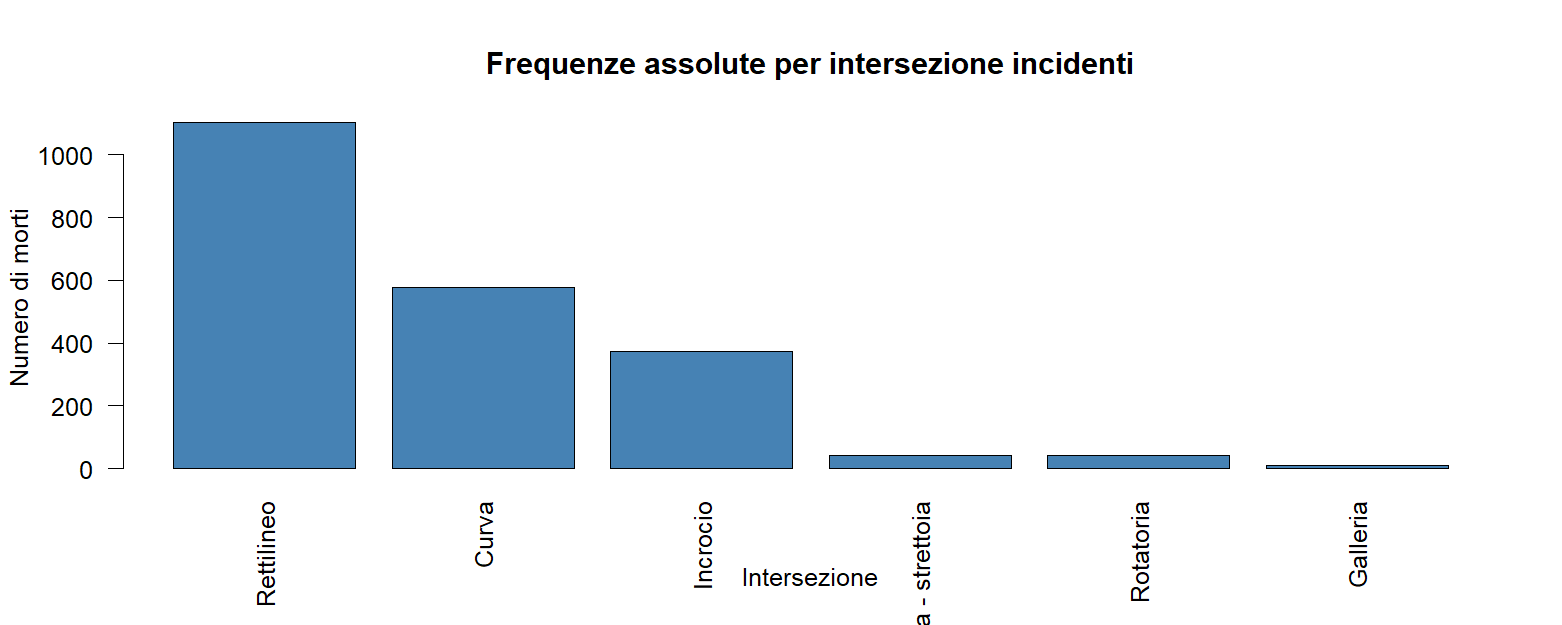
\includegraphics[width=12cm, height=7cm]{Rplot.png} % Adatta l'immagine alla larghezza del testo
\end{figure}

\begin{center}
\begin{lstlisting}[breaklines=true]
# 2. Grafico frequenze relative
barplot(freq_assolute$Frequenza_Relativa, 
        names.arg = freq_assolute$Intersezione,
        main = "Frequenze Relative per Intersezione",
        xlab = "",
        ylab = "",
        col = "coral",
        las = 2,
        cex.names = 0.8)
\end{lstlisting}  
\end{center}

\begin{figure}[H] % H forza la posizione esatta
    \centering
    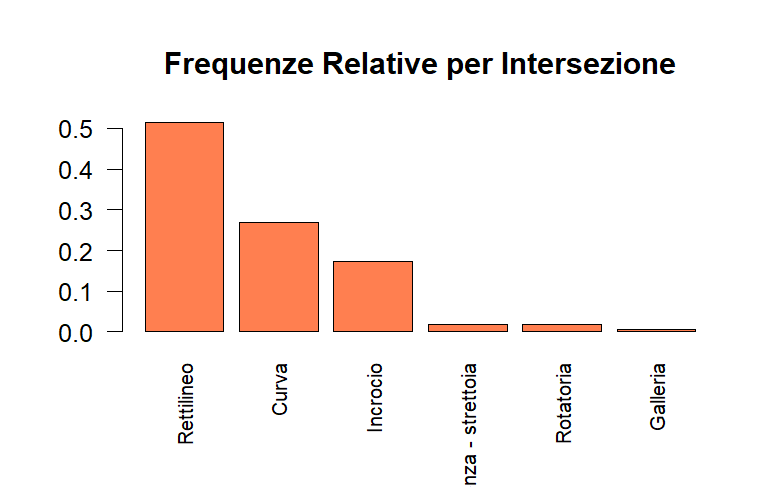
\includegraphics[width=12cm, height=7cm]{Rplot03.png} % Adatta l'immagine alla larghezza del testo
\end{figure}

\begin{center}
\begin{lstlisting}[breaklines=true]
# 3. Grafico frequenze cumulate assolute
barplot(freq_assolute$Frequenza_Cumulata_Assoluta, 
        names.arg = freq_assolute$Intersezione,
        main = "Frequenze Cumulate Assolute",
        xlab = "",
        ylab = "",
        col = "darkgreen",
        las = 2,
        cex.names = 0.8)
\end{lstlisting}  
\end{center}

\begin{figure}[H] % H forza la posizione esatta
    \centering
    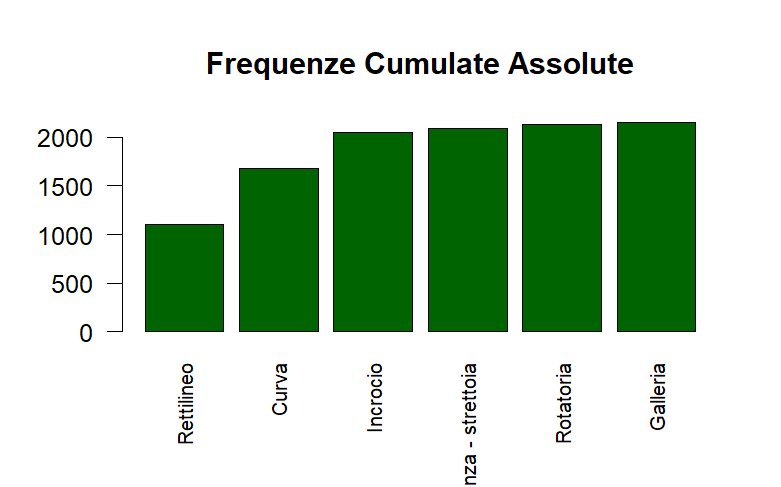
\includegraphics[width=12cm, height=7cm]{Rplot04.png} % Adatta l'immagine alla larghezza del testo
\end{figure}

\begin{center}
\begin{lstlisting}[breaklines=true]
# 4. Grafico frequenze cumulate relative
barplot(freq_assolute$Frequenza_Cumulata_Relativa, 
        names.arg = freq_assolute$Intersezione,
        main = "Frequenze Cumulate Relative",
        xlab = "",
        ylab = "",
        col = "purple",
        las = 2,
        cex.names = 0.8)
\end{lstlisting}  
\end{center}

\begin{figure}[H] % H forza la posizione esatta
    \centering
    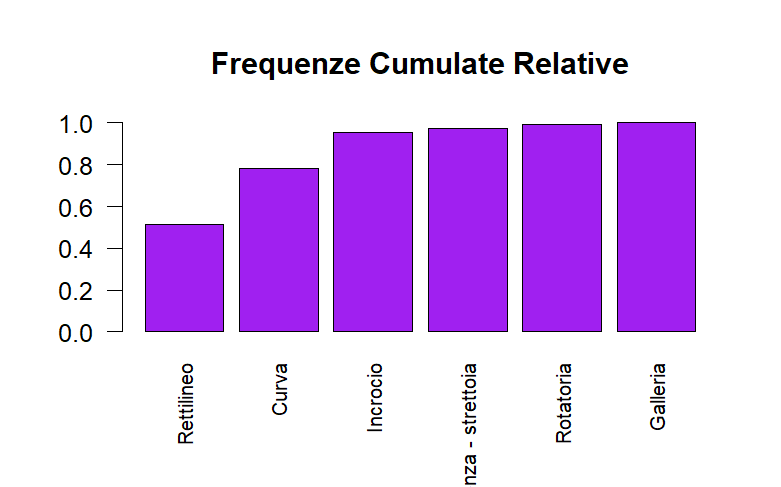
\includegraphics[width=12cm, height=7cm]{Rplot05.png} % Adatta l'immagine alla larghezza del testo
\end{figure}


\begin{center}
\begin{lstlisting}[breaklines=true]
# Converti TIME_PERIOD in fattore per mantenere l'ordine originale
dati$TIME_PERIOD <- factor(dati$TIME_PERIOD, levels = unique(dati$TIME_PERIOD))

# Calcola il numero totale di morti per anno
morti_per_anno <- dati %>%
  group_by(TIME_PERIOD) %>%
  summarise(Totale_Morti = sum(Osservazione, na.rm = TRUE))

# Crea il grafico a linee con tutti gli anni visibili
ggplot(morti_per_anno, aes(x = TIME_PERIOD, y = Totale_Morti, group = 1)) +
  geom_line(color = "steelblue", size = 1) +
  geom_point(color = "steelblue", size = 2) +
  labs(title = "Andamento del numero di morti per incidenti stradali",
       x = "Anno",
       y = "Numero di morti") +
  theme_minimal() +
  theme(plot.title = element_text(hjust = 0.5),
        axis.text.x = element_text(angle = 45, hjust = 1, size = 8)) +  # Riduci dimensione testo
  scale_x_discrete(breaks = levels(morti_per_anno$TIME_PERIOD))  # Mostra tutti i valori
\end{lstlisting}  
\end{center}

\begin{figure}[H] % H forza la posizione esatta
    \centering
    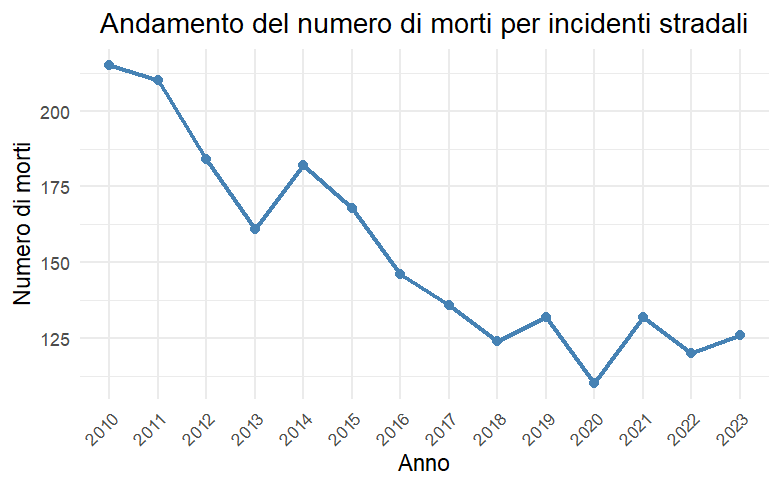
\includegraphics[width=12cm, height=7cm]{Rplot01.png} % Adatta l'immagine alla larghezza del testo
\end{figure}



\chapter{Indici di posizione}
In questo capitolo verranno calcolati gli indici di posizione 
sulla variabile numerica \texttt{Osservazione} del dataset 
\texttt{dati}. \\\\
\noindent
Questa variabile rappresenta il numero di morti
 registrato per una specifica combinazione di tipo di intersezione 
 e anno, limitatamente alla fascia di età dei conducenti tra 21 e 24 
 anni. 

\section{Media campionaria}
La media campionaria è la somma di tutte le osservazioni divisa per il numero di osservazioni.
 Fornisce una misura del valore centrale della distribuzione.
\begin{center}
\begin{lstlisting}[breaklines=true]
media_generale <- mean(dati$Osservazione, na.rm = TRUE)
print(paste("Media campionaria generale delle osservazioni:", round(media_generale, 2)))
\end{lstlisting}  
\end{center}
\noindent
Output: 
\begin{verbatim}
"Media campionaria generale delle osservazioni: 27.51"
\end{verbatim}
Questo valore indica che, in media, per ogni specifica combinazione di tipo di intersezione e anno considerata nel dataset filtrato, si sono registrati circa 27.51 decessi.

\section{Mediana campionaria}
La mediana è il valore centrale di un insieme di dati ordinati.
 Divide i dati in due metà: il 50\% delle osservazioni ha un valore
  inferiore o uguale alla mediana, e il 50\% ha un valore superiore
   o uguale. È meno sensibile ai valori estremi rispetto alla media.

\begin{center}
\begin{lstlisting}[breaklines=true]
mediana_generale <- median(dati$Osservazione, na.rm = TRUE)
print(paste("Mediana generale delle osservazioni:", mediana_generale))
\end{lstlisting}  
\end{center}
\noindent
Output:
\begin{verbatim}
"Mediana generale delle osservazioni: 15.5"
\end{verbatim}
Metà delle combinazioni intersezione/anno hanno registrato 15.5 morti 
o meno, e l'altra metà 15.5 morti o più. Il fatto che la mediana (15.5)
 sia inferiore alla media (27.51) suggerisce una distribuzione 
 asimmetrica a destra.


\section{Moda campionaria}
La moda è il valore (o i valori, in caso di distribuzioni multimodali)
 che appare più frequentemente in un insieme di dati.
\begin{center}
\begin{lstlisting}[breaklines=true]
find_mode <- function(x) {
    u <- unique(x)
    tab <- tabulate(match(x, u))
    u[tab == max(tab)]
  }

find_mode(dati)
\end{lstlisting}  
\end{center}
\noindent
Output: 


\chapter{Indici di variabilità} 
Di seguito calcoliamo gli indici di variabilità, che descrivono la 
variabilità dei dati osservati e consentono di valutare l'informazione 
fornita dall'indice di posizione utilizzato, dando dei dati più accurati.

\section{Varianza campionaria}
La varianza campionaria ($s^2$) misura la dispersione
 media quadratica dei dati attorno alla media campionaria.
  È espressa nell'unità di misura dei dati al quadrato.
\begin{center}
\begin{lstlisting}[breaklines=true]
# Calcolo della varianza sulla variabile 'Osservazione'.
varianza_campionaria <- var(dati$Osservazione, na.rm = TRUE)
print(paste("Varianza campionaria delle osservazioni:", round(varianza_campionaria, 2)))
\end{lstlisting}
\end{center}
\noindent
Output (valore basato sulla media e mediana fornite, è una stima):
\begin{verbatim}
"Varianza campionaria delle osservazioni: 859.52" 
\end{verbatim}
Un valore elevato della varianza indica una notevole
 dispersione dei dati attorno alla media.
    
\section{Deviazione standard campionaria}
La deviazione standard campionaria ($s$) è la radice quadrata 
della varianza campionaria. Fornisce una misura della dispersione
 media dei dati attorno alla media, espressa nella stessa unità 
 di misura dei dati originali, rendendola più interpretabile 
 della varianza.
\begin{center}
\begin{lstlisting}[breaklines=true]
# Calcolo della deviazione standard sulla variabile 'Osservazione'.
dev_std_campionaria <- sd(dati$Osservazione, na.rm = TRUE)
print(paste("Deviazione standard campionaria delle osservazioni:", round(dev_std_campionaria, 2)))
\end{lstlisting}
\end{center}
\noindent
Output (radice quadrata della varianza stimata):
\begin{verbatim}
"Deviazione standard campionaria delle osservazioni: 29.61"
\end{verbatim}
Questo valore indica che, mediamente, i singoli conteggi di 
decessi si discostano dalla media campionaria (27.51) di 
circa 29.61 unità.
    
\section{Scarto medio assoluto}
Lo scarto medio assoluto (Mean Absolute Deviation, MAD)
 dalla media è la media delle deviazioni assolute (cioè, senza segno)
  dei dati dalla loro media. Come la deviazione standard, 
  misura la dispersione media, ma è meno sensibile ai valori 
  anomali perché non eleva al quadrato gli scarti.
\begin{center}
\begin{lstlisting}[breaklines=true]
# Calcolo dello scarto medio assoluto dalla media per 'Osservazione'.
media_oss <- mean(dati$Osservazione, na.rm = TRUE)
scarto_medio_assoluto <- mean(abs(dati$Osservazione - media_oss), na.rm = TRUE)
print(paste("Scarto medio assoluto (dalla media) delle osservazioni:", round(scarto_medio_assoluto, 2)))
\end{lstlisting}
\end{center}
\noindent
Output (stima):
\begin{verbatim}
"Scarto medio assoluto (dalla media) delle osservazioni: 25.13"
\end{verbatim}
In media, le osservazioni si discostano (in valore assoluto) 
dalla media di circa 25.13 decessi.

\section{Ampiezza del campo di variazione}
L'ampiezza del campo di variazione (o semplicemente "range") 
è la differenza tra il valore massimo e il valore minimo osservato 
nel dataset. È una misura di variabilità semplice ma molto sensibile 
ai valori estremi.
\begin{center}
\begin{lstlisting}[breaklines=true]
# Calcolo del minimo, massimo e ampiezza del campo di variazione per 'Osservazione'.
min_oss <- min(dati$Osservazione, na.rm = TRUE)
max_oss <- max(dati$Osservazione, na.rm = TRUE)
ampiezza_variazione <- max_oss - min_oss 

print(paste("Valore minimo delle osservazioni:", min_oss))
print(paste("Valore massimo delle osservazioni:", max_oss))
print(paste("Ampiezza del campo di variazione delle osservazioni:", ampiezza_variazione))
\end{lstlisting}
\end{center}
\noindent
Output:
\begin{verbatim}
"Valore minimo delle osservazioni: 1" 
"Valore massimo delle osservazioni: 102" 
"Ampiezza del campo di variazione delle osservazioni: 101"
\end{verbatim}


\section{Coefficiente di variazione}
Il coefficiente di variazione (CV) è una misura di variabilità relativa,
 data dal rapporto tra la deviazione standard e la media (in valore assoluto).
\begin{center}
\begin{lstlisting}[breaklines=true]
# Calcolo del coefficiente di variazione per 'Osservazione'.
media_oss <- mean(dati$Osservazione, na.rm = TRUE)
dev_std_oss <- sd(dati$Osservazione, na.rm = TRUE)
coeff_variazione <- (dev_std_oss / abs(media_oss)) * 100 # abs() per media se potesse essere negativa
print(paste("Coefficiente di variazione delle osservazioni:", round(coeff_variazione, 2), "%"))
\end{lstlisting}
\end{center}
\noindent
Output(in percentuale):
\begin{verbatim}
"Coefficiente di variazione delle osservazioni: 107.6 %"
\end{verbatim}
Un CV del 107.6\% indica una variabilità molto elevata rispetto alla 
media. Questo è coerente con il fatto che la deviazione standard (29.61)
 è addirittura leggermente superiore alla media (27.51), suggerendo una
  notevole eterogeneità nei conteggi dei decessi.
\FloatBarrier


\chapter{Indici di forma}
 
\section{Indice di asimmetria}

\section{Indice di curtosi} 



\end{document}